\chapter{Analyser}
\label{chp:Analyser}
The flash analyser now outputs values at 125Hz, which is a mixture of various lights and noise. The next step is to create an activity detection algorithm to convert the incoming samples in a logical value: Activity detected or no activity detected. This chapter is separated in three parts. The first part shows what signals are received by the photodiode. The second part explains what methods considered to remove unwanted signals from the signal. The final part of this chapter shows all considerations for the threshold algorithm.

\section{Received signals}
In an ideal world, the system 


\begin{equation}
\label{eq:Pd_light}
PD = I_{L} \alpha + \sum_{i=1}^n I_{Edc_{n}} \beta_{n} + \sum_{i=1}^n I_{Eac{_n}} \gamma_{n} + N_{50Hz} + N(\mu,\sigma^2)
\end{equation}

The goal of the complete algorithm is to isolate $\alpha$ and detect significant changes in real time. It might be possible to create a post-time algorithm with overall better detection rates, but that would be unusable for this usecase.

\section{Filter methods}
The goal of the filters is to get rid of unwanted signals in order to make the detection of $\alpha$ easier.

\subsection{Digital filters}
Digital filters can be used to remove or at least reduce signals we are not interested.

\subsubsection{highpass filters}
Highpass filters can be used to remove $I_{Edc_{n}}$ from the signal.

The highpass filter can ruin the the signal if chosen poorly.

\subsubsection{Lowpass filters}
Lowpass filters can be used to remove $I_{Eac{_n}}$ and $N_{50Hz}$ from the signal.

The Lowpass filter is unable to grantee the removal of $I_{Eac{_n}}$ because of possible aliasing.

\subsection{Moving average filters}
A moving average can be used to reduce $N(\mu,\sigma^2)$ and the remaining $F_allias$.



\subsection{Differential filter}
The differential filter makes use of the signal received when the light is turned off. $PD_{dark}$ can then be subtracted from PD remove several noise sources of the equation.

\begin{equation}
\label{eq:Pd_dark}
PD_{dark} = \sum_{i=1}^n I_{Edc_{n}} \beta_{n} + \sum_{i=1}^n I_{Eac{_n}} \gamma_{n} + N_{50Hz} + N(\mu,\sigma^2)
\end{equation}

\begin{equation}
\label{eq:Pd_light_dark}
PD - PD_{dark} = I_{L} \alpha + N(0,\sigma^2 + \sigma^2_{dark})
\end{equation}

$PD - PD_{dark}$ does not work well with the current hardware set-up as the $PD_{dark}$ is outside the range of the system.

\section{Threshold determination}
The goal of the threshold is to separate significant from insignificant changes in the signal. The challenge in creating a good threshold equation for this problem lies in the variety of signals the system has to deal with. 

\subsection{Naive thresholds methods}

\subsection{Standard deviation based threshold}
A threshold can be made based on the standard deviation of the signal. This method in literature is called the blabla method \cite{@}.

A delay can be added between the threshold and X, to increase detection ratio and detecting speed.

If the delay is too long it might increase the false positive ratio if the signal is slowly drifting upwards.

\subsection{Variance based threshold}
A threshold can be made based on the variance. By comparing 

\section{Algorithm overview}


The first step in creating a proper algorithm, is to identify what signals are affecting the measurements. For this reason, equation \ref{eq:Pd_light} was devised. It shows the composition of the received signal \textbf{$PD$} after it's down sampled to 125Hz with the method described in section \ref{chp:Flash_Analysis}. The equation for $PD$ helps to understand what steps are required to create a reliable algorithm.



The first part of the equation, "\textbf{$ I_{L} \alpha$}", is the amount of light generated by our luminaire ($I_{L}$), multiplied by some factor describing the environment from the point of view of the luminaire ($\alpha$). This signal typically occurs in two ways. The first is an object passing by. The other way this signal can occur is if an object moves into range of the sensor, stops, and then stays still for a long time. This can be modelled as a sine wave, followed by constant, interrupting the wave. The wave is typically a low frequency signal between 0.25Hz and 2Hz (see section \ref{sec:Model}). An example of this signal can be seen in figure \ref{fig:SepparatedSignals}.

The second part of the equation, "\pmb{$\sum_{i=1}^n I_{Edc_{n}} \beta_{n}$}", describes the impact of all constant light sources ($I_{Edc_{n}}$), multiplied by the factor describing the environment from their point of view ($\beta$). An example of a constant light source is moonlight. The final factor involving light in the equation is \pmb{$\sum_{i=1}^n I_{Eac_{n}} \gamma_{n}$}. This describes all fluctuating light sources ($I_{Eac_{n}}$), multiplied once again by an environment describing factor from it's point of view ($\gamma_{n}$). This signal is typically 100Hz as most "old" lights blink or fluctuate at this frequency. Note that the sampling frequency is not twice as big as the sampled frequency, thus aliasing will occur at 25Hz ($= |F_{s} * 1 - F_{Analyze}| = 125 - 100 = 25Hz$)\cite{aliassing}. An example of these signals can be seen in figure \ref{fig:SepparatedSignals}.

The last two terms in the equation have nothing to do with light, but represent noise from all other sources. \pmb{$N_{50Hz}$} represents specifically 50Hz noise. This is powerline-noise picked up by the physical wire of connecting the photo-diode to the amplifier. Normally, line-noise is barely noticeable, but as all the signals are amplified by a 1000 times, it becomes a significant disturbance. The final part of the equation, \pmb{$N(\mu,\sigma^2)$}, is all the noise described in section \ref{subsec:noise}. An example of these signals can be seen in figure \ref{fig:SepparatedSignals}.

The only part of equation \ref{eq:PD} that holds information we can use is $I_{L} \alpha$, or more specifically, the changes of $\alpha$. For this reason, each of the methods described in this section focus on removing the other parts of the equation, or making changes of $\alpha$ more detectable.


\subsection{Removing high frequency components}
\label{subsec:removeing_AC}
Filtering higher frequencies from a signal is a common challenge in signal processing. The signals we try to isolate ($I_{L}\alpha$, 0.25 to 2Hz) are far removed from the frequencies we are trying to suppress ($I_{Eac}$ at 100Hz and $N_{50Hz}$ at 50Hz). The most common method of doing this is by using digital filters. As only the lower frequencies are interesting, a low-pass filter seems to be ideal in this case. There is however one problem. $2 * I_{Eac}$ Is above our sampling frequency, and thus aliasing will occur. In this example it will appear as a 25Hz signal. This signal poses no real issue, as its still an order of magnitude away from the frequency of $ I_{L} \alpha$, and it can still be filtered with a steeper filter. This however, is not always the case in the real world. Any light manufacturer can create lights running at any frequency, and thus there is no guarantee that there won't be a light out there in the world, that can mess the algorithm up. In all other cases this filter probably works fine. Figure \ref{fig:FilterVSAllias} shows how a low-pass filter would remove the signals from the data.

%\begin{figure}
%	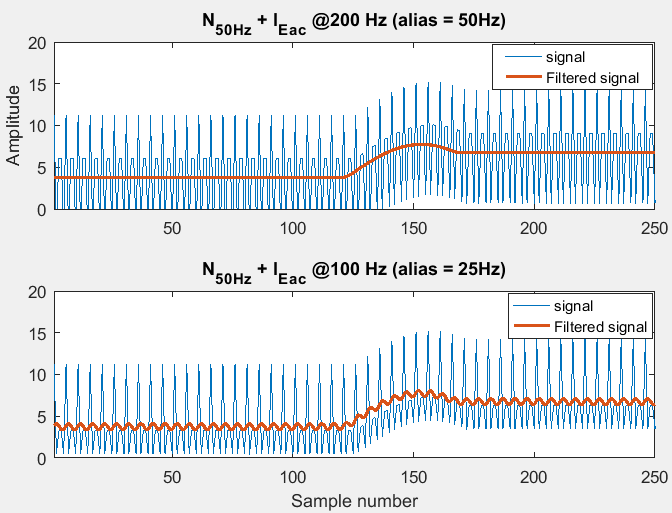
\includegraphics[width=\textwidth]{pics/FirFilter_vs_allias.png}
%	\caption{A low-pass filter, filtering the $I_{Eac}$ and $N_{50Hz}$ signals.}
%	\label{fig:FilterVSAllias}
%\end{figure}

A completely other method of removing these high frequency components is the "$PD_{dark}$" method. This method uses the fact that the sensor set-up can do more than just sampling when the light ($I_{L}$) is turned on. It's also possible to take samples when the light is turned off. The components in such a sample are shown in equation \ref{eq:Pd_dark}. If this sample is obtained a short time away from the original $PD$ then the 50Hz and 100Hz values are roughly the same. Therefore subtracting $PD_{dark}$ from $PD$ gives the equation \ref{eq:Pd_light_dark}, resulting in a signal where $I_{Eac}$, $I_{Edc}$ and $N_{50Hz}$ have practically disappeared.


The signals can't be filtered completely with this method though. This is because of the turn-off time of the LED (see section \ref{sec:Dimming and its consequences}), and the filters used to create a usable signal from the turning on and off of the LED (see section \ref{subsec:T-on_Time}). Both introduce a delay to the $PD_{dark}$ sample. Figure \ref{fig:Phaseshift} shows how much several signals get suppressed at various delay values.

Another downside of this method is that adding or subtracting two noisy signals, leads to signal with even more noise. In this case, an increase of approximately ($\sqrt{\sigma^2+\sigma^2} =$) $\sqrt{2} \sigma$\cite{@needref@}, as the $\sigma$ of $PD$ and $PD_{dark}$ are practically the same.

\begin{figure}
	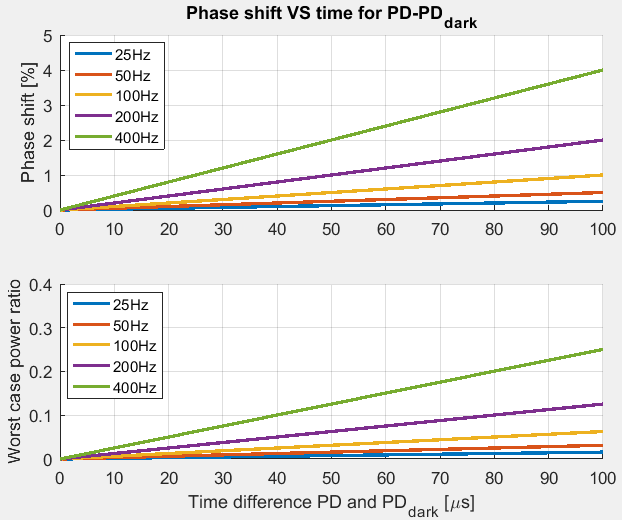
\includegraphics[width=\textwidth]{pics/PasheshiftVStime.png}
	\caption{The amount of phase shift that will occur.}
	\label{fig:Phaseshift}
\end{figure}

The huge selling point of this method in comparison to simply filtering, is that no aliasing of $I_{Eac}$ can occur. Another positive point, is that if a LED is specifically selected for it's a short turn off time, then this filter method is able to remove almost all disturbing sinusoid signals. 

\subsection{Detection threshold}
The first thing necessary to detect changes in $\alpha$ is a change detector, or with other words, if the signal has changed more than $X$, then we assume that the changes in the signal are not caused by noise, but by actual changes of $\alpha$ (the environment). from this point it is assumed that $I_{Eac}$ and $N_{50Hz}$ are no longer a significant part of the signal, as they can be practically removed by any of the methods described in section \ref{subsec:removeing_AC}.

A naive solution to this problem would be to sample a set amount of values when there are no objects in sight. Then, take the maximum and minimum of the sampled values and if the signal ever moves out of the range of the found values, activity is detected. Even though this might work consistently in a dark room (lab environment with no lights), it fails to work in a more realistic environment. If we for example introduce a slowly rising $I_{Edc}$ (e.g. moonlight), then the signal will eventually peak above the current maximum value and trigger a false detection.

Another way of tackling this problem would be to allow the minimum and maximum thresholds to move up and down with the mean of the signal. This results in two thresholds moving up and down together with the mean of the signal, and therefore ignores the slow changing $I_{Edc}$. The downside of this solution is that if the noise level ($N(\mu,\sigma^2)$) where to increases, then the signal would still cross the set threshold and trigger a false detection. The opposite is also true. If the noise level decreases, then the threshold would not scale back automatically and thus making it "deaf" to smaller changes in the signal.

This problem can be solved using the standard deviation of the signal as thresholds instead. A standard deviation scales up and down based on the deviation from the mean, meaning that if a lot of noise is present in the signal, then the detection borders would scale up and vice versa. The detection borders could be set on $\mu\pm T\sigma$, where $\mu$ is the mean, $\sigma$ is the standard deviation and $T$ is a factor determining width of the threshold

Using this method has another benefit. As the noise in our system ($N(\mu,\sigma^2)$) can be approximated with a normal curve (see section \ref{subsec:noise}), it allows us to control the amount of false positives perceived by the system by adjusting the $T$ parameter. How $T$ influences the chance of a false positive can be seen in table \ref{tab:Tresholds}.

\begin{table}
	\centering
	\label{tab:Tresholds}
	\begin{tabular}{cccl}
		\hline
		T   & Chance false positive & Single occurrence @125 Hz & Double occurrence @125Hz\\ \hline
		2   & 4.550026\%            & 0.18s                     & 0.69 days               \\
		3   & 0.269979\%            & 2.96s                     & 198.5 days              \\
		4   & 0.006334\%            & 126.3s                    & 1001 years              \\
		5   & 0.000057\%            & 1178.2s                   & 12199827 years          \\ \hline
	\end{tabular}
	\caption{Chance of a false positive occurring for several values of T, how often this would happen}
\end{table}



%Discuss fixed threshold
%note that this does not adjust to a slowly changing I_DC
%discuss variable threshold with mu and sigma
%show that this kind of works.
%show how scaling m influcences algorithem

\begin{figure}
	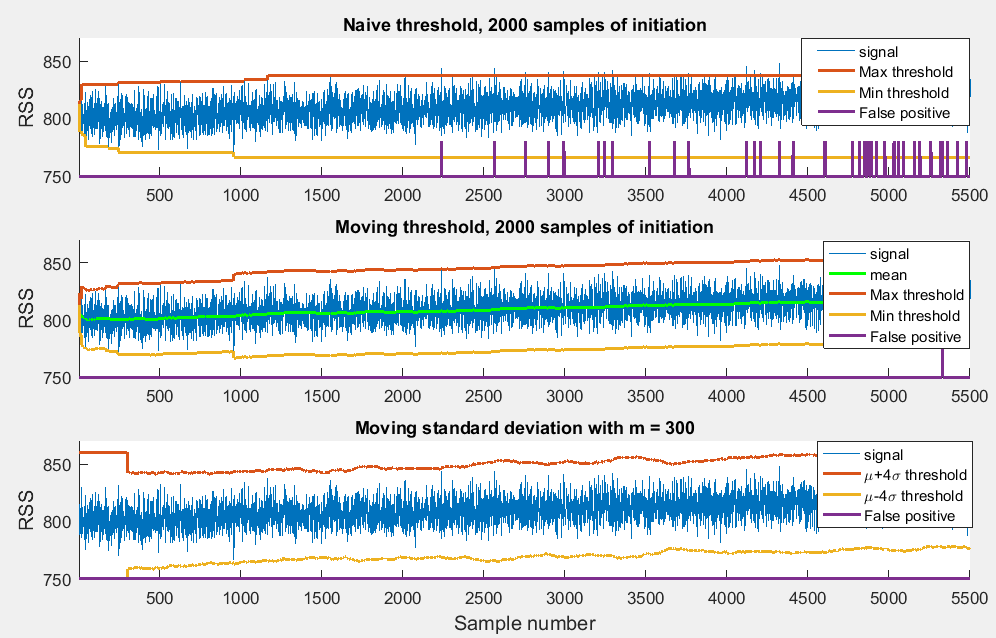
\includegraphics[width=\textwidth]{pics/NaiveVSsigmaThreshold.png}
	\caption{An example of how the discussed threshold algorithms respond to a slowly rising noisy signal.}
	\label{fig:Threshold}
\end{figure}

\subsection{Noise reduction}
The final thing that needs to be done, to make the algorithm more 

Averager \cite{Confidence_interval}

Scaling averager \cite{Confidence_interval}

\begin{figure}
	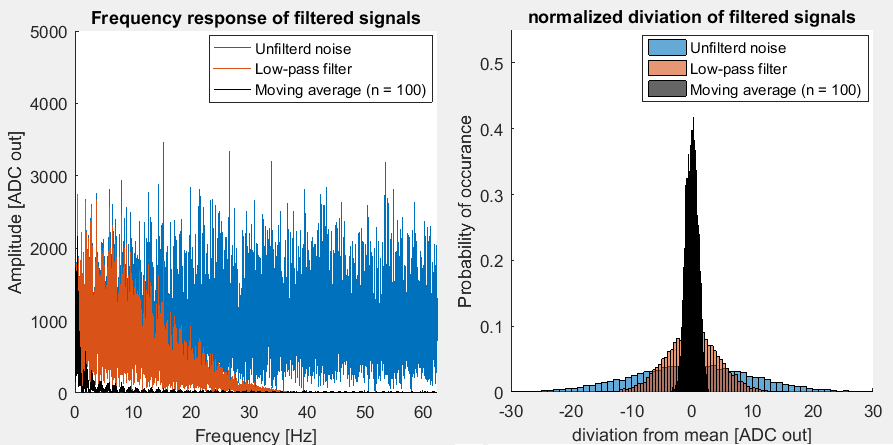
\includegraphics[width=\textwidth]{pics/FiltersVsNoise.png}
	\caption{Frequency response of the noise, the noise when filtered with a low-pass filter, and then noise when filtered with a moving average.}
	\label{fig:FilterVsNoise}
\end{figure}

\begin{equation}
\label{eq:SNR}
SNR = 1 = \frac{\mu * ss}{T * \frac{\sigma}{\sqrt{n}}} \Rightarrow n = \left(\frac{T * \sigma}{\mu*ss}\right)^2
\end{equation}

\begin{equation}
\label{SNR_2}
T * \frac{\sigma}{\sqrt{n}} = \mu * ss
\end{equation}




\subsection{Algorithm overview}
\begin{table}
	\centering
	\label{tab:Filters_summarized}
	\begin{tabular}{lllll}
		\hline
		Algorithm             &\vline $I_{Edc_{n}} \beta_{n}$ & $I_{Eac{_n}} \gamma_{n}$           & $N_{50Hz} $     & $N(\mu,\sigma^2)$    \\ \hline
		Low-pass filter       &\vline None                    & Removed (unless unfortunate alias) & Removed      & Reduced              \\
		$PD - PD_{dark}$      &\vline Removed                 & Removed                            & Removed         & $\sqrt2$ increase    \\
		Moving average        &\vline None                    & Reduced                            & Reduced         & Statistically reduced\\
		Scaling moving average&\vline None                    & Greatly reduced                    & Greatly reduced & Statistically reduced\\ \hline
	\end{tabular}
	\caption{Overview of all decent filter algorithms with their effects on each signal.}
\end{table}

\begin{figure}
	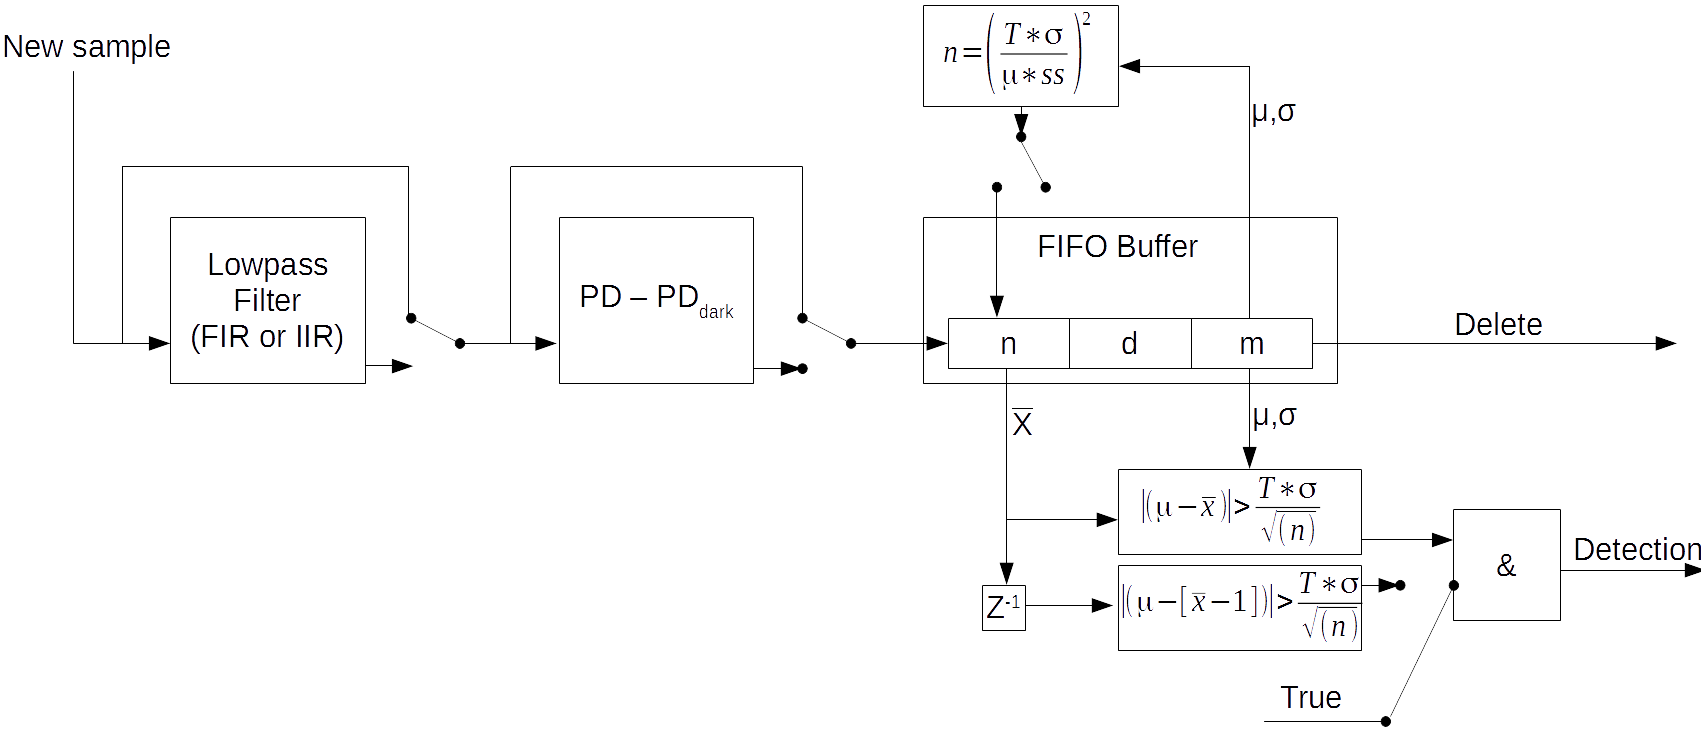
\includegraphics[angle=90,width=\textwidth]{pics/allSTDbasedAlgorithms_expanded.png}
	\caption{Overview of the algorithm.}
	\label{fig:fullAlgorithm}
\end{figure}
